%================================================================
\chapter{Quantum Machine Learning}\label{chap:QML}
%================================================================
Over the years, many different quantum algorithms have been proposed that is anticipated to greatly outshine classical methods. Perhaps most famously is the Shor's algorithm\cite{Shor_1997}, which promises to factor integers in polynomial time. This is is believed to be an exponentially hard problem for classical computers. However, such useful quantum algorithms often need a large number of error-corrected qubits to be efficient, meaning noise introduced by the environment and inaccuracy of the gates is corrected for. Also, their implementation requires often a large number of quantum gates, requiring the quantum computer to handle deep circuits. As explained in \autoref{sec:Nisq}, near-term quantum computers are not able to accommodate these criteria, and are thus unsuitable. What would then be some interesting candidate algorithms for useful near-term applications? A promising family of algorithms are \emph{parameterized quantum circuits}(PQC), which are quantum circuits comprised of fixed gates, such as CNOT gates, and adjustable gates, such as Pauli rotations\cite{Benedetti_2019}. Unlike algorithms that are tailored to solve specific problems, such as Shor's algorithm for factoring integers, PQCs are general algorithms with free parameters that needs to be adjusted in order to solve a given problem. In practice, quantum computers are used to evaluate the circuits, while classical hardware is used to post-process the results and optimized the parameters. In this sense, both quantum and classical hardware are leveraged to solve the problem in a variational manner. This hybrid approach is though to be much less demanding on the number qubits and the depth of the circuit, as much of the computation is outsource to classical computers\cite{Cerezo_2021}. Thus, they are much more suitable for near-term applications. Moreover, since PQC are not problem specific, one is freed from the need to tailor algorithms for solving specific problems, which is otherwise hard in practice because of how non-intuitive quantum computing can be. 

Lately, there has been a lot of research on the use of PQC as machine learning models, often called \emph{Quantum Neural Network}(QNN)\cite{abbas2020power}\cite{Benedetti_2019}. In general, the typical structure of QNNs can be broken up into three stages: \emph{feature encoding}, \emph{processing} and \emph{measurement} with potential post-processing. This general procedure is summarized in \autoref{fig:QNN}.

\begin{figure}[htp]
\[ \begin{array}{c}
    \Qcircuit @C=1em @R=1em {
    \lstick{\ket{0}}& \multigate{3}{{U_{\phi(\boldsymbol{x})}}} & \qw & \multigate{3}{U_{\boldsymbol{\theta}}}  & \qw &  \qw  & \meter  & z_1\\
    \lstick{\ket{0}}& \ghost{{U_{\phi(\boldsymbol{x})}}} & \qw & \ghost{U_{\boldsymbol{\theta}}}  & \qw &  \qw  & \meter  & z_2\\
    \vdots & \nghost{{U_{\phi(\boldsymbol{x})}}} & \vdots  & \nghost{U_{\boldsymbol{\theta}}}  & \vdots &   &   & \\
    \lstick{\ket{0}}& \ghost{{U_{\phi(\boldsymbol{x})}}} & \qw & \ghost{U_{\boldsymbol{\theta}}}  & \qw &  \qw  & \meter  & z_n\\
    & \underset{Encoding}{\underbrace{}}&&\underset{Processing}{\underbrace{}}&&&\underset{Measurement}{\underbrace{}}
    }
    \end{array} \rightarrow \underset{Estimation}{\underbrace{\hat{y} = \bra{\psi_{\boldsymbol{x}, \boldsymbol{\theta}}} \hat{O} \ket{\psi_{\boldsymbol{x}, \boldsymbol{\theta}}}}}\]
\caption{The general structure of a Quantum Neural Network(QNN). The procedure consists of three steps: A routine $\ket{\psi_{\boldsymbol{x}}} = U_{\phi(\boldsymbol{x})}\ket{0}$ for encoding a feature vector onto an n-qubit Hilbert space. Next, $\ket{\psi_{\boldsymbol{x}, \boldsymbol{\theta}}} = U_{\boldsymbol{\theta}}$ applies a unitary transformation parameterized by $\boldsymbol{\theta}\ket{\psi_{\boldsymbol{x}}}$, transforming the state in Hilbert space. Lastly, the expectation value of some appropriate observable $\hat{O}$ is estimated for the resulting state, yielding in a model output $\hat{y} = \bra{\psi_{\boldsymbol{x}, \boldsymbol{\theta}}} \hat{O} \ket{\psi_{\boldsymbol{x}, \boldsymbol{\theta}}}$.}
\label{fig:QNN}
\end{figure}

The QNN starts by encoding a feature vector $\boldsymbol{x}$ onto a $n$-qubit Hilbert space by using a unitary transformation 
\begin{equation}
    \ket{\psi_{\boldsymbol{x}}} = U_{\phi(\boldsymbol{x})}\ket{\boldsymbol{0}},
\end{equation}
often called a \emph{quantum feature map}. Next, a circuit parameterized by $\boldsymbol{\theta} = (\theta_1, \cdots, \theta_{n_{\theta}})$ is applied, resulting in 
\begin{equation}
    \ket{\psi_{\boldsymbol{x}, \boldsymbol{\theta}}} = U_{\boldsymbol{\theta}}\ket{\psi_{\boldsymbol{x}}}.
\end{equation} In this context, this circuit $U_{\boldsymbol{\theta}}$ is often called an \emph{ansatz} and serves as a general way of transforming the state $\ket{\psi_{\boldsymbol{x}}}$ encoding the data in Hilbert space. Lastly, the expectation value of some appropriate observable $\hat{O}$ is estimated for this state, resulting in a model output 
\begin{equation}\label{eq:QNN}
    \hat{y} = f_{QNN}(\boldsymbol{x};\boldsymbol{\theta}) = \bra{\psi_{\boldsymbol{x}, \boldsymbol{\theta}}} \hat{O} \ket{\psi_{\boldsymbol{x}, \boldsymbol{\theta}}}.
\end{equation} In the standard approach of supervised learning, the parameters $\boldsymbol{\theta}$ must be adjusted in order to minimize some loss function $L(\boldsymbol{\theta}) = \frac{1}{N}\sum_{i=1}^N L(\hat{y_i},y_i)$, as explained in \autoref{sec:ParametricModels}. 

In the sections to come, we will discuss specific choices of feature encoding, ansätze, and expectation values.

%================================================================
\section{Feature Encoding}\label{sec:FeatureEncoding}
%================================================================
In this section, we will introduce two ways of doing feature encoding, namely \emph{qubit encoding}, \emph{RZZ encoding}. 

%================================================================
\subsection{Qubit Encoding}\label{sec:QubitEncoding}
%================================================================
One popular approach for encoding a feature vector to a quantum state is the often-called method \emph{qubit encoding}\cite{Benedetti_2019}. This encoding requires $p$ qubits, where $p$ is the number of features, and it can be applied at a constant circuit depth. Before the encoding, the data is optionally pre-processed by some function $\phi(x_i)$, for example scaling of the data. Then, the encoding works by performing a Pauli-rotation on each qubit with a rotational angle equal to the corresponding (pre-processed) feature. \autoref{fig:qubitencoding} shows how qubit encoding is implemented using $R_x$, $R_y$ and $R_z$ rotation.

\begin{figure}[H]
     \begin{subfigure}[b]{0.3\textwidth}
         \centering
         \[\Qcircuit @C=1em @R=.7em {
         \lstick{\ket{0}}& \gate{R_x(\phi(x_1))} &  \qw \\
         \lstick{\ket{0}}& \gate{R_x(\phi(x_2))} &  \qw \\
         \vdots&  &   \\
         \lstick{\ket{0}}& \gate{R_x(\phi(x_p))} &  \qw
         }\]
     \end{subfigure}
     \hfill
     \begin{subfigure}[b]{0.3\textwidth}
         \centering
         \[\Qcircuit @C=1em @R=.7em {
         \lstick{\ket{0}}& \gate{R_y(\phi(x_1))} &  \qw \\
         \lstick{\ket{0}}& \gate{R_y(\phi(x_2))} &  \qw \\
         \vdots&  &   \\
         \lstick{\ket{0}}& \gate{R_y(\phi(x_p))} &  \qw
         }\]
     \end{subfigure}
     \hfill
     \begin{subfigure}[b]{0.3\textwidth}
         \centering
         \[\Qcircuit @C=1em @R=.7em {
         \lstick{\ket{0}}& \gate{H}& \gate{R_z(\phi(x_1))} &  \qw \\
         \lstick{\ket{0}}&\gate{H}& \gate{R_z(\phi(x_2))} &  \qw \\
         \vdots& & &  \\
         \lstick{\ket{0}}&\gate{H}& \gate{R_z(\phi(x_p))} &  \qw
         }\]
     \end{subfigure}
        \caption{Qubit encoding using $R_x$, $R_y$ and $R_z$ rotations to encode $p$ features, left to right. $\phi(\cdot)$ applies some kind of pre-processing to the samples, e.g. scaling.}
        \label{fig:qubitencoding}
\end{figure}

When using $R_z$ rotations, a Hadamard gate is used on each qubit to create a super-position, as these rotations would otherwise leave $\ket{\boldsymbol{0}}$ invariant. As an example, two features $\boldsymbol{x} = (x_1, x_2)$ can be qubit encoded onto two qubits in the following way using $R_y$ rotations:

\begin{equation}
    R_y(x_1)\otimes R_y(x_2) (\ket{0} \otimes \ket{0}) = 
    (\cos(\frac{x_1}{2})\ket{0} + \sin(\frac{x_1}{2})\ket{1})\otimes
    (\cos(\frac{x_2}{2})\ket{0} + \sin(\frac{x_2}{2})\ket{1})
\end{equation}
Writing the tensor product out as an explicit state vector, we get 

\begin{equation}\label{eq:qubit rotation interaction}
\begin{bmatrix}
    \cos(\frac{x_1}{2})\cos(\frac{x_2}{2}) \\
    \cos(\frac{x_1}{2})\sin(\frac{x_2}{2}) \\
    \sin(\frac{x_1}{2})\cos(\frac{x_2}{2}) \\
    \sin(\frac{x_1}{2})\sin(\frac{x_2}{2}) \\
    \end{bmatrix}.
\end{equation}
We see from this that qubit encoding provides a state whose amplitudes encode interactions between the features. In this sense, it computes an exponential number of interactions between features in constant time, potentially creating a powerful representation of the data useful for solving a give learning problem.


As the the number of features are increased, the number of amplitudes will increase exponentially and contribute higher and higher interactions, creating a complex representation of the data in Hilbert space. 

As the circuit depth is quite low, qubit encoding is an effective method for embedding $p$ features into a $2^p$ dimensional Hilbert space. However, the state resulting from qubit encoding is mathematically very simple, which may limit the overall expressive power of the final model. In the next subsection, we will present a more complex way of encoding features which has been shown to improve the overall flexibility of the machine learning model in some circumstances. 


%================================================================
\subsection{Tensorial Feature Mapping}\label{sec:Tensorial Feature Mapping}
%================================================================

From \autoref{eq:qubit rotation interaction}, we see that qubit encoding computes interactions between the features. This observation can be used to create interesting representations for data of few features by repeating them multiple times, at the expense of including more qubits. By imposing $x_1 = x_2 = x$ in the example in \autoref{sec:QubitEncoding}

\begin{equation}\label{eq:tensorial feature mapping}
\begin{bmatrix}
    \cos(\frac{x}{2})^2 \\
    \sin(\frac{x}{2})\cos(\frac{x}{2}) \\
    \sin(\frac{x}{2})\cos(\frac{x}{2}) \\
    \sin(\frac{x}{2})^2 \\
    \end{bmatrix}.
\end{equation}

This technique is sometimes called  \emph{tensorial feature mapping}(kilde), and results in a state that encodes polynomials of $\sin$ and $\cos$ transformations of data, as seen in \autoref{eq:tensorial feature mapping}. In (kilde), tensorial feature mapping was shown to produce superior QNN models over normal qubit encoding. 


%================================================================
\subsection{RZZ Encoding}\label{sec:RZZencoding}
%================================================================
\citet{abbas2020power} implemented a quantum feature map for encoding quantum features up to second order, meaning the embedding is dependent on terms such as $x_i x_j$, for $i\neq j$. The method can be seen as an extension of qubit encoding using $R_z$ gates, with additional extra RZZ gates that act on qubit $i$ and $j$ with rotational angle $\phi(x_i, x_j) = (\pi - x_i)(\pi - x_j)$. This is done for $i\in [1, \cdots, p-1]$ and $j\in [i+1, \cdots, p]$. As this way of encoding was never given a name, we will call it \emph{RZZ encoding} in this thesis. The circuit implementing RZZ encoding can be seen in \autoref{fig:Rzzencoding}

\begin{figure}[H]
    \centering
    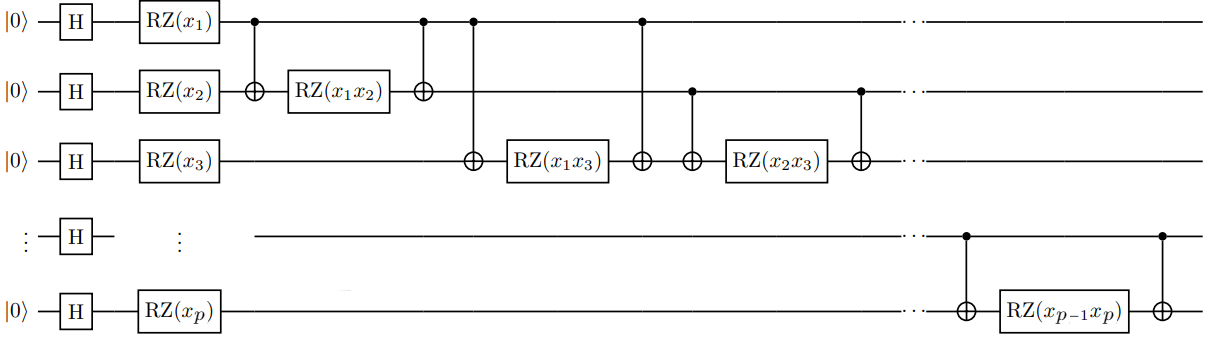
\includegraphics[width=14cm]{latex/figures/Rzz_encoding.png}
    \caption{Circuit visualizing implementation of RZZ encoding of $p$ features. The figure is retrieved from \cite{abbas2020power} and adapted to fit our notation.}
    \label{fig:Rzzencoding}
\end{figure}

This procedure produces a much more complex feature map, and can be made more complex still by repeating the whole encoding process several times in a row. The number of such repetitions is often called the \emph{depth} of the feature map.  \citet{abbas2020power} conjecture that this feature map is difficult to simulate classically for depth $\geq 2$ and increasing number of features. Since it requires $\mathcal{O}(p^2)$ operations on a quantum computer, its time complexity is polynomial and hence efficient in comparison. It was showed by the same authors that RZZ encoding produce much more flexible models than qubit encoding. However, it is also more computationally demanding, as it requires a circuit depth $\mathcal{O}(p^2)$ and full connectivity between all the qubits.

%================================================================
%\subsection{Amplitude Encoding}\label{sec:AmplitudeEncoding}
%================================================================
%\emph{Amplitude encoding} is a way of encoding features directly as the amplitudes of a quantum state. Given a data set $\boldsymbol{x} = (x_1, \cdots, x_p)$, where $p=2^n$, amplitude encoding involves preparing a state $\ket{\psi_\boldsymbol{x}} = \sum_{i=1}^p x_i\ket{i}$ on $n$ qubits. Because of the normalization of quantum states, it is necessary to scale the data to ensure that $\sum_{i=1}^p |x_i|^2 = 1$ holds. The main advantage of amplitude encoding stems from the fact that the number of amplitudes is exponential in the number of qubit. Hence, we only need $\log_2(p)$ qubits to encode $p$ features, enabling us to encode an exponential amount of information as the number of qubits increase. However, there is not a general way of preparing a state for any given $\boldsymbol{x} = (x_1, \cdots, x_p)$ in an efficient way, i.e. with time-complexity polynomial in the number of qubits.

%Here, we will present a method for preparing an arbitrary state $\ket{\psi}$ with real-valued amplitudes starting from the initial state $\ket{0}$. The method is based on the description of \cite{SupervisedwquantumComputers}, which is in turn based on the work of \cite{Mottonen}. The method prepares the state by iterativly \emph{branching} the state by using multi-controlled rotations. Consider a general system of $n$ qubits. Starting in the state $\ket{00\cdots0}$ the algorithm applies an $R_y$ rotation with rotation angle $\beta^1_1$ on the first qubit
%\begin{equation}
%    \ket{\psi_1} = R_y^1(\beta^1_1)\ket{000} = a_1\ket{00\cdots0} + a_2\ket{10\cdots0},
%\end{equation}
%where the superscript of the gate indicates which qubit it acts on. 
%This creates two different branches where the first qubit is in state $\ket{0}$ and $\ket{1}$, respectively. Then, for each branch, we apply a different rotation on the second qubit. This can be done by conditioning the rotation on the first qubit, resulting in  
%\begin{equation}
%\begin{aligned}
%    \ket{\psi_2} = R_y^{2|q_1 = 0}(\beta^2_1)R_y^{2|q_1 = 1}(\beta^2_2)\ket{\psi_1} =\\ a_1(b_1\ket{00\cdots0} + b_2\ket{01\cdots0}) + a_2(b_3\ket{10\cdots0} + b_4\ket{11\cdots0}).
%\end{aligned}
%\end{equation}
%Here, the superscript "$2|q_1=0$" means that the gate is applied on the second qubit, conditioned on the first qubit being in state $\ket{0}$ ($q_1=0$). 
%In this way, each branch is broken into two new branches. This procedure is continued until all possible branches has been created. In general, we use multi-controlled rotations on qubit $i$ conditioned on all possible states of the preceding qubits, i.e.
%\begin{equation}
%    R_y^{i|q_1,\cdots,q_{i-1}}(\beta^i_j)\ket{q_1 \cdots q_{i-1}}\otimes \ket{0},
%\end{equation}
%where $j$ enumerates the $2^{i-1}$ different branches of $\ket{q_1 \cdots q_{i-1}}$. To ensure that we arrive at the desired amplitude after all the branches have been created, we must choose rotation angles

%\begin{equation}
%    \beta^{i}_j = 2\arcsin{
%    \frac{\sqrt{\sum_{l=1}^{2^{n-i}} |x_{(2j - %1)2^{n-i} + l}|^2}}
%    {\sqrt{\sum_{l=1}^{2^{n-i+1}} |x_{(j-1)2^{n-i+1}  %+ l}|^2}}
%    },
%\end{equation}
%with the special case for $i=n$

%\begin{equation}
%    \beta^{n}_j = 2\arcsin{
%    \frac{x_{(2j - 1) + l}}
%    {\sqrt{\sum_{l=1}^{2} |x_{2(j-1)  + l}|^2}}
%    }.
%\end{equation}
%As an easy example, lets say we want to encode the normalized features $\boldsymbol{x} = %(x_1, x_2, x_3 ,x_4)$ onto two qubits. We start by calculating the first rotation angle:
%\begin{equation}
%    \beta^{(1)}_1 = 2\arcsin{
%    \frac{\sqrt{|x_3|^2 + |x_4|^2}}{\sqrt{|x_1|^2 + |x_2|^2 + |x_3|^2 + |x_4|^2}}
%    } = 2\arcsin{\sqrt{|x_3|^2 + |x_4|^2}},
%\end{equation}
%where the normalization of the vector was used to remove the denominator. 

%The full procedure is visualized in the following circuit:

%\begin{equation}
%   \Qcircuit @C=1em @R=.7em {
%         \lstick{\ket{0}}& \gate{R_y(\beta^{1}_1)}&  \ctrl{1}                  & \ctrlo{1}                 & \qw &  \qw    &  \ctrl{1}                 & \ctrlo{1}                 &  \qw    &  \ctrlo{1}                        &\\
%         \lstick{\ket{0}}& \qw                      &  \gate{R_y(\beta^{2}_1)} & \gate{R_y(\beta^{2}_2)} & \qw &  \qw    &  \ctrl{2}                 & \ctrl{2}                  &  \qw    &  \ctrlo{2}                        &\\
%         \vdots          &                          &                            &                           &     &  \cdots &                           &                           &  \cdots &                                   &\\
%         \lstick{\ket{0}}& \qw                      &  \qw                       & \qw                       & \qw &  \qw    &  \ctrl{1}                 & \ctrl{1}                  &  \qw    &  \ctrlo{1}                        &\\
%         \lstick{\ket{0}}& \qw                      &  \qw                       & \qw                       & \qw &  \qw    &  \gate{R_y(\beta^{n}_1)}& \gate{R_y(\beta^{n}_2)} &  \qw    &  \gate{R_y(\beta^{n}_{2^{n-1}})} &\\
%         }        
%\end{equation}



    


%================================================================
\section{Ansätze}\label{sec:Ansätze}
%================================================================
What kind of unitary transformation are interesting as ansätze used for processing information embedded in quantum states? In principle, we are able to explore every conceivable unitary transformation as a parameterized circuit, since there are circuit designs that are known to be \emph{universal}\cite{lloyd2018quantum}. In this context, universality means that for any unitary operator, there exists a sufficiently deep ansatz that approximates the operator to an arbitrary accuracy. However, such approximations are often exponentially deep\cite{NielsenQuantum}, meaning the vast majority of unitary transformations are inaccessible on ideal quantum computers, let alone near-term quantum computers. Still, it is believed that there exists reasonably shallow ansatz that are useful for constructing powerful machine learning models. Many of these ansätze are also believed to be classically hard to simulate, eluding to a possible quantum advantage for quantum machine learning\cite{lloyd2020quantum}.

In this thesis, we will investigate an ansatz that respect limitations of near-team quantum computers, focusing on circuit depth that scales linearly with the number of qubits and linear connectivity between qubits. We will refer to this ansatz as the \emph{simple ansatz}(SA). It can be visualised as 

\begin{equation}
U_{SA}(\boldsymbol{\theta}) = 
\begin{array}{c}
\Qcircuit @C=1.5em @R=.7em {
        &       \ctrl{1} & \qw       &  \qw      &  \qw      & \gate{R_y(\theta_1)}&\\
        &       \targ    & \ctrl{1}  &  \qw      &  \qw      & \gate{R_y(\theta_2)}&\\
        &       \qw      & \targ     &  \ctrl{0} &  \qw      & \gate{R_y(\theta_3)}&\\
        &       \vdots   &  \vdots         &  \vdots   &\vdots   & \vdots  \\
        &       \qw      & \qw       &  \qw      &  \targ    &\gate{R_y(\theta_{n_{\theta}})}&  \\
         }
\end{array}.
\end{equation}
The simple ansatz applies CNOT gates on neighboring qubits in sequence until the final qubit is reached. This creates entanglement between the qubits and enables access to a larger space of transformations, as explained in \autoref{sec:ControlledOperations}. Then, an $R_y$ rotation is applied to each qubit, each parameterized with its own parameter. Both the number of parameters and the circuit depth of the simple ansatz scales linearly with the number of qubits, making it hardware-efficient and hopefully suitable for near-term applications. 

In order to produce a more expressive ansatz, we may repeat the simple ansatz $d$ number of times with independent parameter as such:

\begin{equation}\label{eq:simple ansatz}
    \ket{\psi_{\boldsymbol{x}, \boldsymbol{\theta}}} = 
    U_{SA}(\boldsymbol{\theta}^r)\cdots U_{SA}(\boldsymbol{\theta}^2) U_{SA}(\boldsymbol{\theta}^1)\ket{\psi_\boldsymbol{x}},
\end{equation}
where $\boldsymbol{\theta}^i$ are independent vectors of parameters. We call $d$ the repetitions of the ansatz.

%================================================================
\section{Inference}\label{sec:Inference}
%================================================================
To derive a model output $\hat{y}$, we must estimate the expectation value of some observable with respect to the state prepared by the encoder and ansatz, i.e. $\hat{y} =\bra{\psi_{\boldsymbol{x},\boldsymbol{\theta}}}
\hat{O} 
\ket{\psi_{\boldsymbol{x},\boldsymbol{\theta}}}$. In the same manner as \cite{abbas2020power}, we use the \emph{parity} of the state to derive a model output for inference. The parity of an $n$ qubit state can be formulated as an operator as
\begin{equation}
    P = \frac{1}{2}(I^{\otimes n} + \bigotimes_{i=1}^n \sigma_z).
\end{equation}
Applying this operator on a computational basis state $\ket{v_1  \cdots v_n}$ computes 


\begin{equation}
    P\ket{v_1  \cdots v_n} = 
    \frac{1}{2}(\ket{v_1  \cdots v_n} -(-1)^{\sum_{i=1}^n v_i}\ket{v_1  \cdots v_2}) = 
    \bigoplus_{i=1}^n v_i \ket{v_1  \cdots v_n}, 
\end{equation}
where $\bigoplus_{i=1}^n v_i$ is the mod 2 sum of the terms $v_i$, also known as the parity of the bitstring $v_1\cdots v_n$. In short, the parity of the state is $0$ if the number of qubits in state $\ket{1}$ is even, and is otherwise 1. This is called even and odd parity, respectively. 

To estimate the expected parity $\bra{\psi_{\boldsymbol{x},\boldsymbol{\theta}}}P 
\ket{\psi_{\boldsymbol{x},\boldsymbol{\theta}}}$, we use the technique described in \autoref{sec:EstimatingExpectationValues} by preparing the state repeatedly and measure it in the computational basis. The expected parity can then be estimated as 

\begin{equation}
    \bra{\psi_{\boldsymbol{x},\boldsymbol{\theta}}}P 
    \ket{\psi_{\boldsymbol{x},\boldsymbol{\theta}}}
    \approx
    \frac{1}{S} \sum_{j=1}^S p_j,
\end{equation}
where $S$ is the number of shots used, and $p_j$ is the parity resulting from measurement $ij$.


%================================================================
\section{Optimization of PQC}\label{sec:OptPQC}
%================================================================
A key component of hybrid methods such as PQC is the optimization of the parameters $\boldsymbol{\theta}$ entering the ansatz. These parameters are usually optimized with respect to some objective function in order to solve a given problem \cite{Benedetti_2019}. In the context of machine learning, one seeks to minimize the loss function \autoref{eq:LossFunction} to fit labeled data. There are multiple popular methods for optimization in the context of PQC. One such method is numerical differentiation of the loss function:

\begin{equation}
    \frac{\partial}{\partial \theta_i} L(\boldsymbol{\theta}) 
    \approx \frac{L(\theta_1, \cdots, \theta_i + \epsilon, \cdots \theta_{n_{\theta}}) - L(\theta_1, \cdots, \theta_i, \cdots \theta_{n_{\theta}})}{\epsilon},
\end{equation}
for a sufficiently small $\epsilon>0$. Having an approximation of the gradient, one can optimize the parameters using gradient descent or similar techniques. However, because of the high amount of noise of near-term quantum computers, finite difference approximations of derivatives can be unfavorable in practise. Recently, analytical techniques have been proved to be very efficient for calculating the gradient on quantum computers \cite{abbas2020power} \cite{Benedetti_2019}. In the next section, we will detail how this gradient can be calculated. 

%================================================================
\subsection{Analytical Gradient-Based Optimization}\label{sec:AnalyticalGrad}
%================================================================
Based on the derivation presented by \cite{Schuld_2019}, we will now present how the gradient of a large class of PQC's can be calculated on quantum computers using the \emph{parameter shift rule}.

Assume we have some circuit parameterized by $\boldsymbol{\theta}$ that prepares a state $\ket{\psi_{\boldsymbol{\theta}}} = U_{\boldsymbol{\theta}}\ket{0}$. The expectation value of some observable $\hat{O}$ can be formulated as 

\begin{equation}
    a = \bra{\psi_{\boldsymbol{\theta}}} \hat{O} \ket{\psi_{\boldsymbol{\theta}}} = \bra{0}U_{\boldsymbol{\theta}}^{\dagger}\hat{O}U_{\boldsymbol{\theta}}\ket{0}.
\end{equation}
Assume for simplicity that any parameter $\theta_i$ affects only a single gate. Then, since any circuit can be decomposed into a sequence of gates, we can decompose the circuit as $U_{\boldsymbol{\theta}}\ket{0} = AG(\theta_i)B$, where $G$ is the only gate dependent on $\theta_i$, and $A$ and $B$ is the rest of the circuit. This allows us to rewrite the expectation value as 

\begin{equation}
    a = \bra{\psi'} G(\theta_i)^{\dagger} \hat{O}' G(\theta_i) \ket{\psi'},
\end{equation}
where $\ket{\psi'} = B\ket{0}$ and $\hat{O}' = A^{\dagger}\hat{O}A$. Starting from this expression, it is easy to compute the derivative of the expectation value:

\begin{equation}
    \partial_{\theta_i} a = \bra{\psi'} G(\theta_i)^{\dagger} \hat{O}' (\partial_{\theta_i}G(\theta_i)) \ket{\psi'} + h.c.,
\end{equation}
where h.c. refers to the hermitian conjugate. In its current form, the terms of above expression cannot be computed on a quantum computer since they don't have the form of expectation values. However, it is possible to rewrite it as a linear combination of two expectation values

\begin{equation}\label{eq:generalDeriv}
\begin{aligned}
    \partial_{\theta_i} a = 
    \frac{1}{4}(
    \bra{\psi'} [G(\theta_i)+2\partial_{\theta_i}G(\theta_i)]^{\dagger} \hat{O}' [G(\theta_i)+2\partial_{\theta_i}G(\theta_i)] \ket{\psi'} -\\
    \bra{\psi'} [G(\theta_i)-2\partial_{\theta_i}G(\theta_i)]^{\dagger} \hat{O}' [G(\theta_i)-2\partial_{\theta_i}G(\theta_i)] \ket{\psi'}).
\end{aligned}
\end{equation}

Are $[G(\theta_i)+2\partial_{\theta_i}G(\theta_i)]$ and $[G(\theta_i)-2\partial_{\theta_i}G(\theta_i)]$ unitary operators? In the case that they are not, it will not possible to implement them as circuits. However, for gates such as Pauli rotations, they turn out to be unitary up to a constant factor and actually quite easy to implement. Given that $G(\theta_i) = R_j(\theta_i) = e^{-i\theta_i \sigma_j/2}$, where $j \in [x,y,z]$, we have that 
\begin{equation}
    G(\theta_i)\pm2\partial_{\theta_i}G(\theta_i) = 
    \underset{\sqrt{2}G(\pm \frac{\pi}{2})}{\underbrace{(I \mp i\sigma_j)}}G(\theta_i) = 
    \sqrt{2}G(\theta_i \pm \frac{\pi}{2}),
\end{equation}
where the relation $R_j(a)R_j(b) = R_j(a+b)$ was used in the last step. Inserting this result back into \autoref{eq:generalDeriv}, we get the final expression 


\begin{equation}\label{eq:parameterShiftRule}
\begin{aligned}
    \partial_{\theta_i} a = 
    \frac{1}{2}(
    \bra{\psi'} G(\theta_i + \frac{\pi}{2})^{\dagger} \hat{O}' G(\theta_i + \frac{\pi}{2}) \ket{\psi'} -\\
    \bra{\psi'} G(\theta_i - \frac{\pi}{2}) \hat{O}' G(\theta_i - \frac{\pi}{2}) \ket{\psi'}).
\end{aligned}
\end{equation}

The form of the above expression reveals the origin of the name "parameter shift rule". To calculate the derivative of the expectation value of a circuit, one simply has to estimate this expectation value twice: Once with the corresponding parameter shifted by $\frac{\pi}{2}$, and once shifted by $-\frac{\pi}{2}$. The derivative is finally found by combining the two results in a linear combination. This is a very efficient approach for computing the gradient, since the number of expectation values that needs to be estimated is proportional to the number of parameters.

For QNNs, the features $\boldsymbol{x}$ enter the state $\ket{\psi_{\boldsymbol{x},\boldsymbol{\theta}}}$ in the same way as the parameters $\boldsymbol{\theta}$ if qubit encoding is used(see \autoref{sec:QubitEncoding}), i.e. with Pauli rotations. In this case, the parameter shift rule can also be applied to calculate the derivative of the output with respect to the features, i.e. $\partial_{x_i}a$. This will be relevant when we later introduce models consisting of multiple circuits. 

%================================================================
\subsection{Barren Plateus in QNN Loss Landscape}\label{sec:BarrenPlateus}
%================================================================
While recent studies have shown several promising characteristics of QNNs, such as faster training and greater flexibility\cite{abbas2020power}, these studies have been largely focused on smaller systems and heuristic measures. As such, few scaling relations of QNNs have been rigorously proven. Recently, \citet{McClean_2018} established an important result connecting the magnitude of the gradient and observables for a large class of PQCs to the number of qubits. First, they point out that observables of a state $\ket{\psi_n}$ sampled uniformly from an n-qubit Hilbert space tend to concentrate around the its mean over the whole Hilbert space as the number of qubits increases. Mathematically, we can express this as

\begin{equation}
    \lim_{n\to\infty} V(\bra{\psi_n}\hat{O}\ket{\psi_n}) = 0,
\end{equation}
where $V()$ indicates the variance. Also, this concentration happens exponentially fast in n. From \autoref{sec:Ansätze}, we know that a PQC $U_{\boldsymbol{\theta}}$ can in general prepare any state $\ket{\psi_\boldsymbol{\theta}}$ only if it is exponentially deep. However, \citet{McClean_2018} showed that shallow PQC with polynomial depth were also susceptible for the same exponential concentration of observable. This effect is also worsening the deeper the circuit is. Further, they showed that tha gradient of PQC has a mean around zero, i.e.

\begin{equation}
     E(\partial \theta_i \bra{\psi_{\boldsymbol{\theta}}}\hat{O}\ket{\psi_{\boldsymbol{\theta}}}) = 0.
\end{equation}

These two results show that the gradient of PQCs are concentrarting around zero. In other words, as the depth and width of PQCs grows, they essentially approached a random circuit, leading to a concentration of outputs around an the average output over all possible initialization. In addition, their gradients vanish exponentially fast.

The vanishing of PQCs gradients manifests itself as loss landscapes that are extremely flat in most of parameter space, reminiscent of the vanishing gradient phenomenon of classical neural networks as the depth increase\cite{shalevshwartz2017failures}. The exponential vanishing of the gradient means that exponentially many shots are required in order to obtain a sufficient signal-to-noise ratio, as explained in \autoref{sec:EstimatingExpectationValues}. This may render the training of larger QNN models intractable as the number of qubits is increased in order to handle harder learning problems.


%================================================================
\section{Quantum Circuit Network}\label{sec:Quantum Circuit Network}
%================================================================
In order to extend the QNN framework discussed so far, we will implement multi-circuit models that utilize several such QNNs. These models exhibit a network-like structure, consisting of layers of several circuits. The layers of circuits transform feature vectors in a sequential manner until a model prediction is obtained. To avoid confusion with "quantum neural networks", we have opted to call the multi-circuit model a \emph{quantum circuit network}(QCN). This type of architecture was explored by \citet{b} and found to be able to sufficiently fit a nonlinear function in one dimension when optimized with Nelder-Meads algorithm, a gradient-free optimization algorithm.


%================================================================
\subsection{Feed-Forward}\label{sec:FeedForward}
%================================================================
\autoref{fig:QCN} illustrates the general structure of a quantum circuit network, which exhibits neural network-like architecture. Here, each node in the network is a QNN model $f^{(l)}_{QNN}$(see \autoref{eq:QNN}), with some layer specific choice of encoder, ansatz and observable. Each QNN is parameterized by $\boldsymbol{\theta}^{[l,j]}$, where $l$ is the layer and $j$ is the node in the current layer. The feed-forward procedure is described as follows: 
For layer $l$, each node receives the feature vector $\boldsymbol{a}^{(l-1)}$ resulting from the previous layer(with the special case that $\boldsymbol{a}^{(0)} = \boldsymbol{x}$). For each node $j$, an output $a^{(l)}_k$ is produced, i.e.
\begin{equation}
    a^{(l)}_j = f^{(l)}_{QNN}(\boldsymbol{a}^{(l-1)}; \boldsymbol{\theta}^{[l,j]})
\end{equation}
These outputs are then concatenated to make a new feature vector $\boldsymbol{a}^{(l)}$. This is then repeated for each layer $1$ through $L$. Finally, the output of the last is identified as the model output
\begin{equation}\label{eq:QCN}
    \hat{y} = f_{QCN}(\boldsymbol{x}; \boldsymbol{\theta}) = \boldsymbol{a}^{(L)},
\end{equation}
where $\boldsymbol{\theta}$ is the collection of all $\boldsymbol{\theta}^{[l,j]}$.


\begin{figure}[htp]
    \centering
    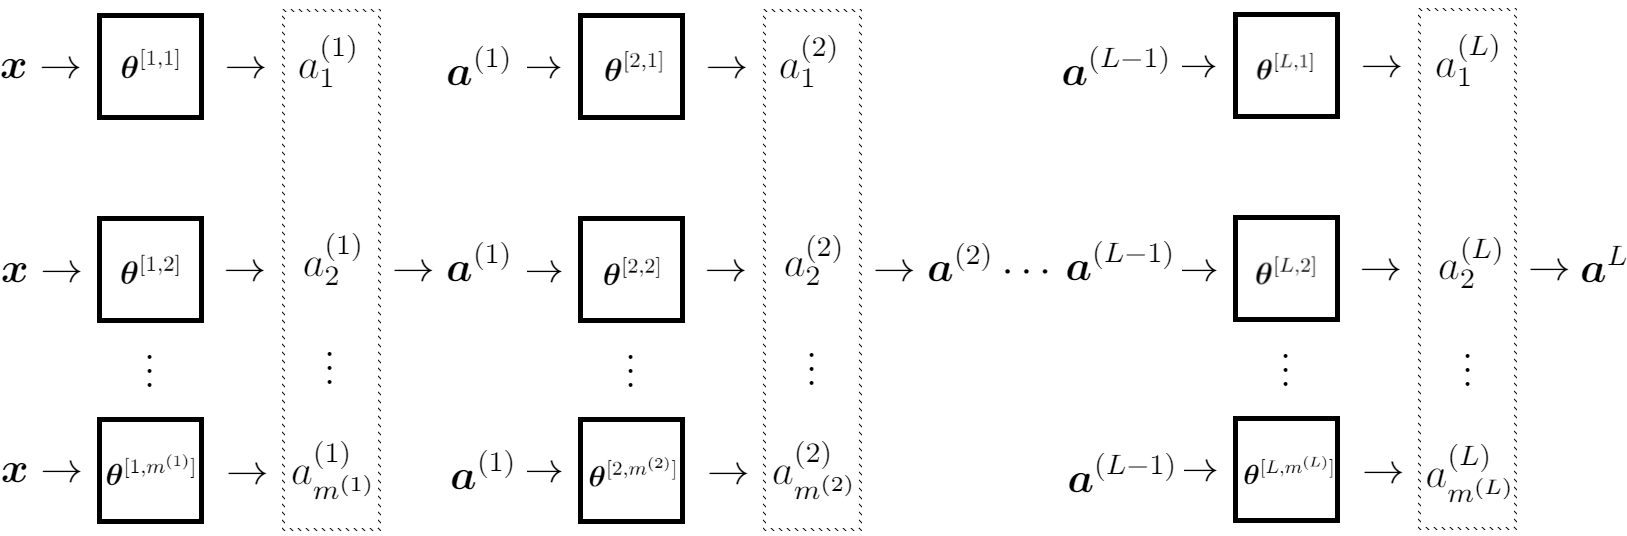
\includegraphics[width = 15cm]{latex/figures/QCN.png}
    \caption{General structure of a quantum circuit network. Each node, indicated by a box, is a QNN model parameterized by $\boldsymbol{\theta}^{[l,j]}$, where $l$ is the layer and $j$ is the node in the current layer. $m^{(l)}$ is the number of nodes in layer $l$. For layer $l$, each node receives the feature vector $\boldsymbol{a}^{(l-1)}$ resulting from the previous layer(with the special case that $\boldsymbol{a}^{(0)} = \boldsymbol{x}$). For each node $j$, an output $a^{(l)}_j$ is produced, which is then concatenated to make a new feature vector $\boldsymbol{a}^{(l)}$. This is then repeated for each layer $1$ through $L$. Finally, the output of the last layer is identified as the model output $\hat{y} = \boldsymbol{a}^{(L)}$.}
    \label{fig:QCN}
\end{figure}

The sequential transformation resulting from the multi-circuit architecture of QCNs offer several interesting properties compared to the single circuit QNN models. First, as the circuits are evaluated one at a time, it is possible to compute very large models of many parameters without the need for quantum computers that can sustain a very long coherence time. While QNNs of many paramaters generally have high circuits depths and consist of many qubits, QCN can on the other hand consist of many more shallow circuits of few qubits, much more suitable for near-term quantum computers. 

Further, the repeated embedding and estimation of outputs of intermediate layers may alter the space of functions possible to compute in an interesting way. This is because each of these steps introduce a nonlinear transformation of the data. For classical neural networks, we know from \autoref{sec:DenseNeuralNetwork} that repeated nonlinear transformation is key for their great expressive power. Switching over to the single-circuit QNN model, nonlinearity is introduced only twice: First when the features are encoded as a quantum state using rotations such as $R_j(x_i)\ket{0} = \cos(\frac{x_i}{2})\ket{0} - i\sin(\frac{x_i}{2})\sigma_j\ket{0}$. The second time is when an output is derived by estimating an expectation value, which relates to the modulo square of the amplitudes of the state, i.e. $|\alpha_k|^2$. All other processing of the data is performed by the ansatz, which by definition is unitary and therefore linear in nature. In this sense, it could be that the formulation of QNNs as shown in \autoref{fig:QNN} could be a bit constrained with respect to what functions it can compute. By combining several circuits, nonlinearity is introduced with each layer, possibly creating a more powerful model able to fit more complicated functions.  



%================================================================
\subsection{Backward Propagation}\label{sec:BackwardPropagationQCN}
%================================================================
Comparing the formulation of QCN \autoref{eq:QCN} and classical neural network \autoref{eq:DNN}, it can be seen that they are structurally the same down to the mathematical operations happening inside each node. For the QCN each node implements a QNN model, while the classical neural network implements an affine transformation, followed by a nonlinear activation. Using this oberservation, it is possible to implement a slightly modified backpropagation, earlier described in \autoref{sec:BackpropogationDNN}, for QCN. This assumes that we are able to calculate the derivative of the outputs of each QNN model. As described in \autoref{sec:ParametricModels}, this is indeed possible using the parameter shift rule. 

For $\hat{y} = f_{QCN}(\boldsymbol{x}; \boldsymbol{\theta})$ and a loss function $L(\hat{y}, y)$, the error of the last layer can be computed as 
\begin{equation}\label{eq:lastLayerErrorQCN}
    \delta^L_k = \frac{\partial L(\hat{y}, y)}{\partial \boldsymbol{a}^L_k},
\end{equation}
where $k$ indicates the node. This error can be defined for any layer recursively by repeated application of the chain-rule:
\begin{equation}\label{eq:errorQCN}
    \delta^l_j = \frac{\partial L(\hat{y}, y)}{\partial \boldsymbol{a}^l_j} 
    = \sum_k \frac{\partial L(\hat{y}, y)}{\partial \boldsymbol{a}^{l+1}_k} \frac{\partial \boldsymbol{a}^{l+1}_k}{\partial \boldsymbol{a}^{l}_j}
    = \sum_k \delta^{l+1}_k \frac{\partial \boldsymbol{a}^{l+1}_k}{\partial \boldsymbol{a}^{l}_j}.
\end{equation}

The derivative of the loss function with respect to any parameter in any node can then be calculated as 
\begin{equation}\label{eq:derivweightsQCN}
    \frac{\partial L(\hat{y}, y)}{\partial \theta^{[l,j]}_n} = 
    \sum_k \frac{\partial L(\hat{y}, y)}{\partial \boldsymbol{a}^{l}_k} \frac{\partial \boldsymbol{a}^{l}_k}{\partial \theta^{[l,j]}_n} 
    = \delta^l_j \frac{\partial \boldsymbol{a}^{l}_j}{\partial \theta^{[l,j]}_n},
\end{equation}
where it was used that $\frac{\partial \boldsymbol{a}^{l}_k}{\partial \theta^{[l,j]}_n} = 0$ for $k \neq j$, since the output of node $k$ is independent of the parameters in node $j$. 

The terms 
\begin{equation}\label{eq:localGradients}
\begin{aligned}
    \frac{\partial \boldsymbol{a}^{l}_j}{\partial \theta^{[l,j]}_n}, \frac{\partial \boldsymbol{a}^{l+1}_k}{\partial \boldsymbol{a}^{l}_j}
\end{aligned}
\end{equation} are the derivatives of the node outputs with respect to the parameters and inputs, respectively. Since they are calculated locally for each node, we call them the \emph{local gradients} of the QCN model. As explained in \autoref{sec:AnalyticalGrad}, the local gradients can be calculated analytically using the parameter shift rule with respect to the parameters $\theta^{[l,j]}_n$ and the inputs $\boldsymbol{a}^{l}_j$. By first performing a forward pass to calculate $\boldsymbol{a}^{l}$ for all the layers $l$, the local gradients can then estimated and stored one at a time. Finally, \autoref{eq:derivweightsQCN} can be used to classically compute the \emph{total gradient} $\nabla_{\boldsymbol{\theta}} L(\hat{y},y)$ based on the stored values for the single sample $\boldsymbol{x}$. Repeating this for all samples $\boldsymbol{x}^{(i)}$, we can calculate the average total gradient \begin{equation}\label{eq:averageGradientQCN}
    \nabla_{\boldsymbol{\theta}} L(\boldsymbol{\theta}) = \frac{1}{N}\sum_{i=1}^N \nabla_{\boldsymbol{\theta}} L(\hat{y}^{(i)}, y^{(i)}).
\end{equation}  The calculation of the gradient allows us to leverage more information of the loss function and enables for gradient-based optimisation. Potentially, this could mean faster optimization relative to derivative-free optimization, such as Nelder-Mead's algorithm which was originally used to optimize QCN(kilde). However, as explained in \autoref{sec:GradientDescent}, gradient-based methods such as gradient descent are prone to getting stuck in local minima, potentially causing slow optimization.    

%================================================================
\subsection{Regularized Feature Map}\label{sec:Regularized Feature map}
%================================================================

\begin{figure}[htp]
\[ \begin{array}{c}
    \Qcircuit @C=1em @R=1em {
    \lstick{\ket{0}}& \multigate{3}{{U_{\phi(\boldsymbol{x})}}} & \qw    & \multigate{3}{S_{\boldsymbol{\theta}}} & \qw    & \multigate{3}{{U^{-1}_{\phi(\boldsymbol{x})}}} & \qw    &  \\
    \lstick{\ket{0}}& \ghost{{U_{\phi(\boldsymbol{x})}}}        & \qw    & \ghost{S_{\boldsymbol{\theta}}}        & \qw    &\ghost{{U^{-1}_{\phi(\boldsymbol{x})}}}        & \qw    &  \\
    \vdots          & \nghost{{U_{\phi(\boldsymbol{x})}}}       & \vdots & \nghost{S_{\boldsymbol{\theta}}}       & \vdots & \nghost{{U^{-1}_{\phi(\boldsymbol{x})}}}       & \vdots &   \\
    \lstick{\ket{0}}& \ghost{{U_{\phi(\boldsymbol{x})}}}        & \qw    & \ghost{S_{\boldsymbol{\theta}}}        & \qw    &\ghost{{U_{\phi(\boldsymbol{x})}}}        & \qw    &  \\
                    & \underset{Encoder}{\underbrace{}}        &        &\underset{Splitter}{\underbrace{}}    &        &\underset{Reverse  Encoding}{\underbrace{}}        &             
    }
    \end{array}\]
\caption{}
\label{fig:QNN}
\end{figure}



%================================================================
%\section{Recursive Circuit Optimization}\label{sec:RCO}
%================================================================

%Assume we have a unitary operator $U$ that prepares a state$\ket{\psi} = U\ket{0}$. In the case that $U$ has a high circuit depth, preparation of the state may fail on noisy hardware due to decoherence, as explained in \autoref{sec:Nisq}. 

